\subsection{Diseño.}

\subsubsection{Aplicaciones similares.}

En la fase inicial del proceso de diseño se llevó a cabo una revisión de aplicaciones existentes con enfoques similares al planteado, con el objetivo identificar funcionalidades relevantes y oportunidades de mejora que pudieran ser la base de las decisiones de diseño del proyecto. El análisis se concentró en tres launchers de código abierto que compartían la filosofía de minimalismo y funcionalidad enfocada en la productividad:

Hex Launcher \cite{HexLauncher} se destacó por su simplicidad visual y la organización de aplicaciones mediante categorías. Su interfaz limpia proporcionó indicadores sobre cómo reducir la sobrecarga visual sin comprometer la funcionalidad.

Launcher \cite{MinimalLauncher}, por su parte, se enfoca en atajos que sean útiles para acceder a las aplicaciones. Su diseño minimalista y la ausencia de elementos decorativos innecesarios sirvieron como inspiración para la creación de una interfaz que prioriza la funcionalidad sobre la estética.


Olauncher \cite{Olauncher}, contribuyó especialmente en demostrar la efectividad de un diseño extremadamente minimalista centrado en listas textuales en lugar de iconos gráficos para las aplicaciones. Esta aproximación confirmó la viabilidad de eliminar los elementos visuales tradicionalmente asociados con el reconocimiento instantáneo de aplicaciones, reemplazándolos por una interfaz que fomenta el uso consciente e intencional del dispositivo.

\subsubsection{Mockups y prototipo.}

Luego de haber identificado los elementos deseados en la interfaz, se empezaron a diseñar wireframes de baja fidelidad utilizando un tablero físico con marcadores borrables, explorando ideas y cambiando rápidamente los elementos que necesitaran ajustes. Durante estas sesiones, surgieron diversas aproximaciones para la organización de la información, la distribución de elementos en pantalla y los flujos de navegación entre diferentes funcionalidades. Desde el principio se tuvo en cuenta la necesidad de darle protagonismo a las funcionalidades de gestión de tareas y hábitos, ocupando gran parte de la pantalla de inicio con la intención de que el usuario siempre tuviera visible sus pendientes.

\begin{figure}[H]
  \caption{Wireframe en tablero.}
  \label{fig:wireframe_tablero}
  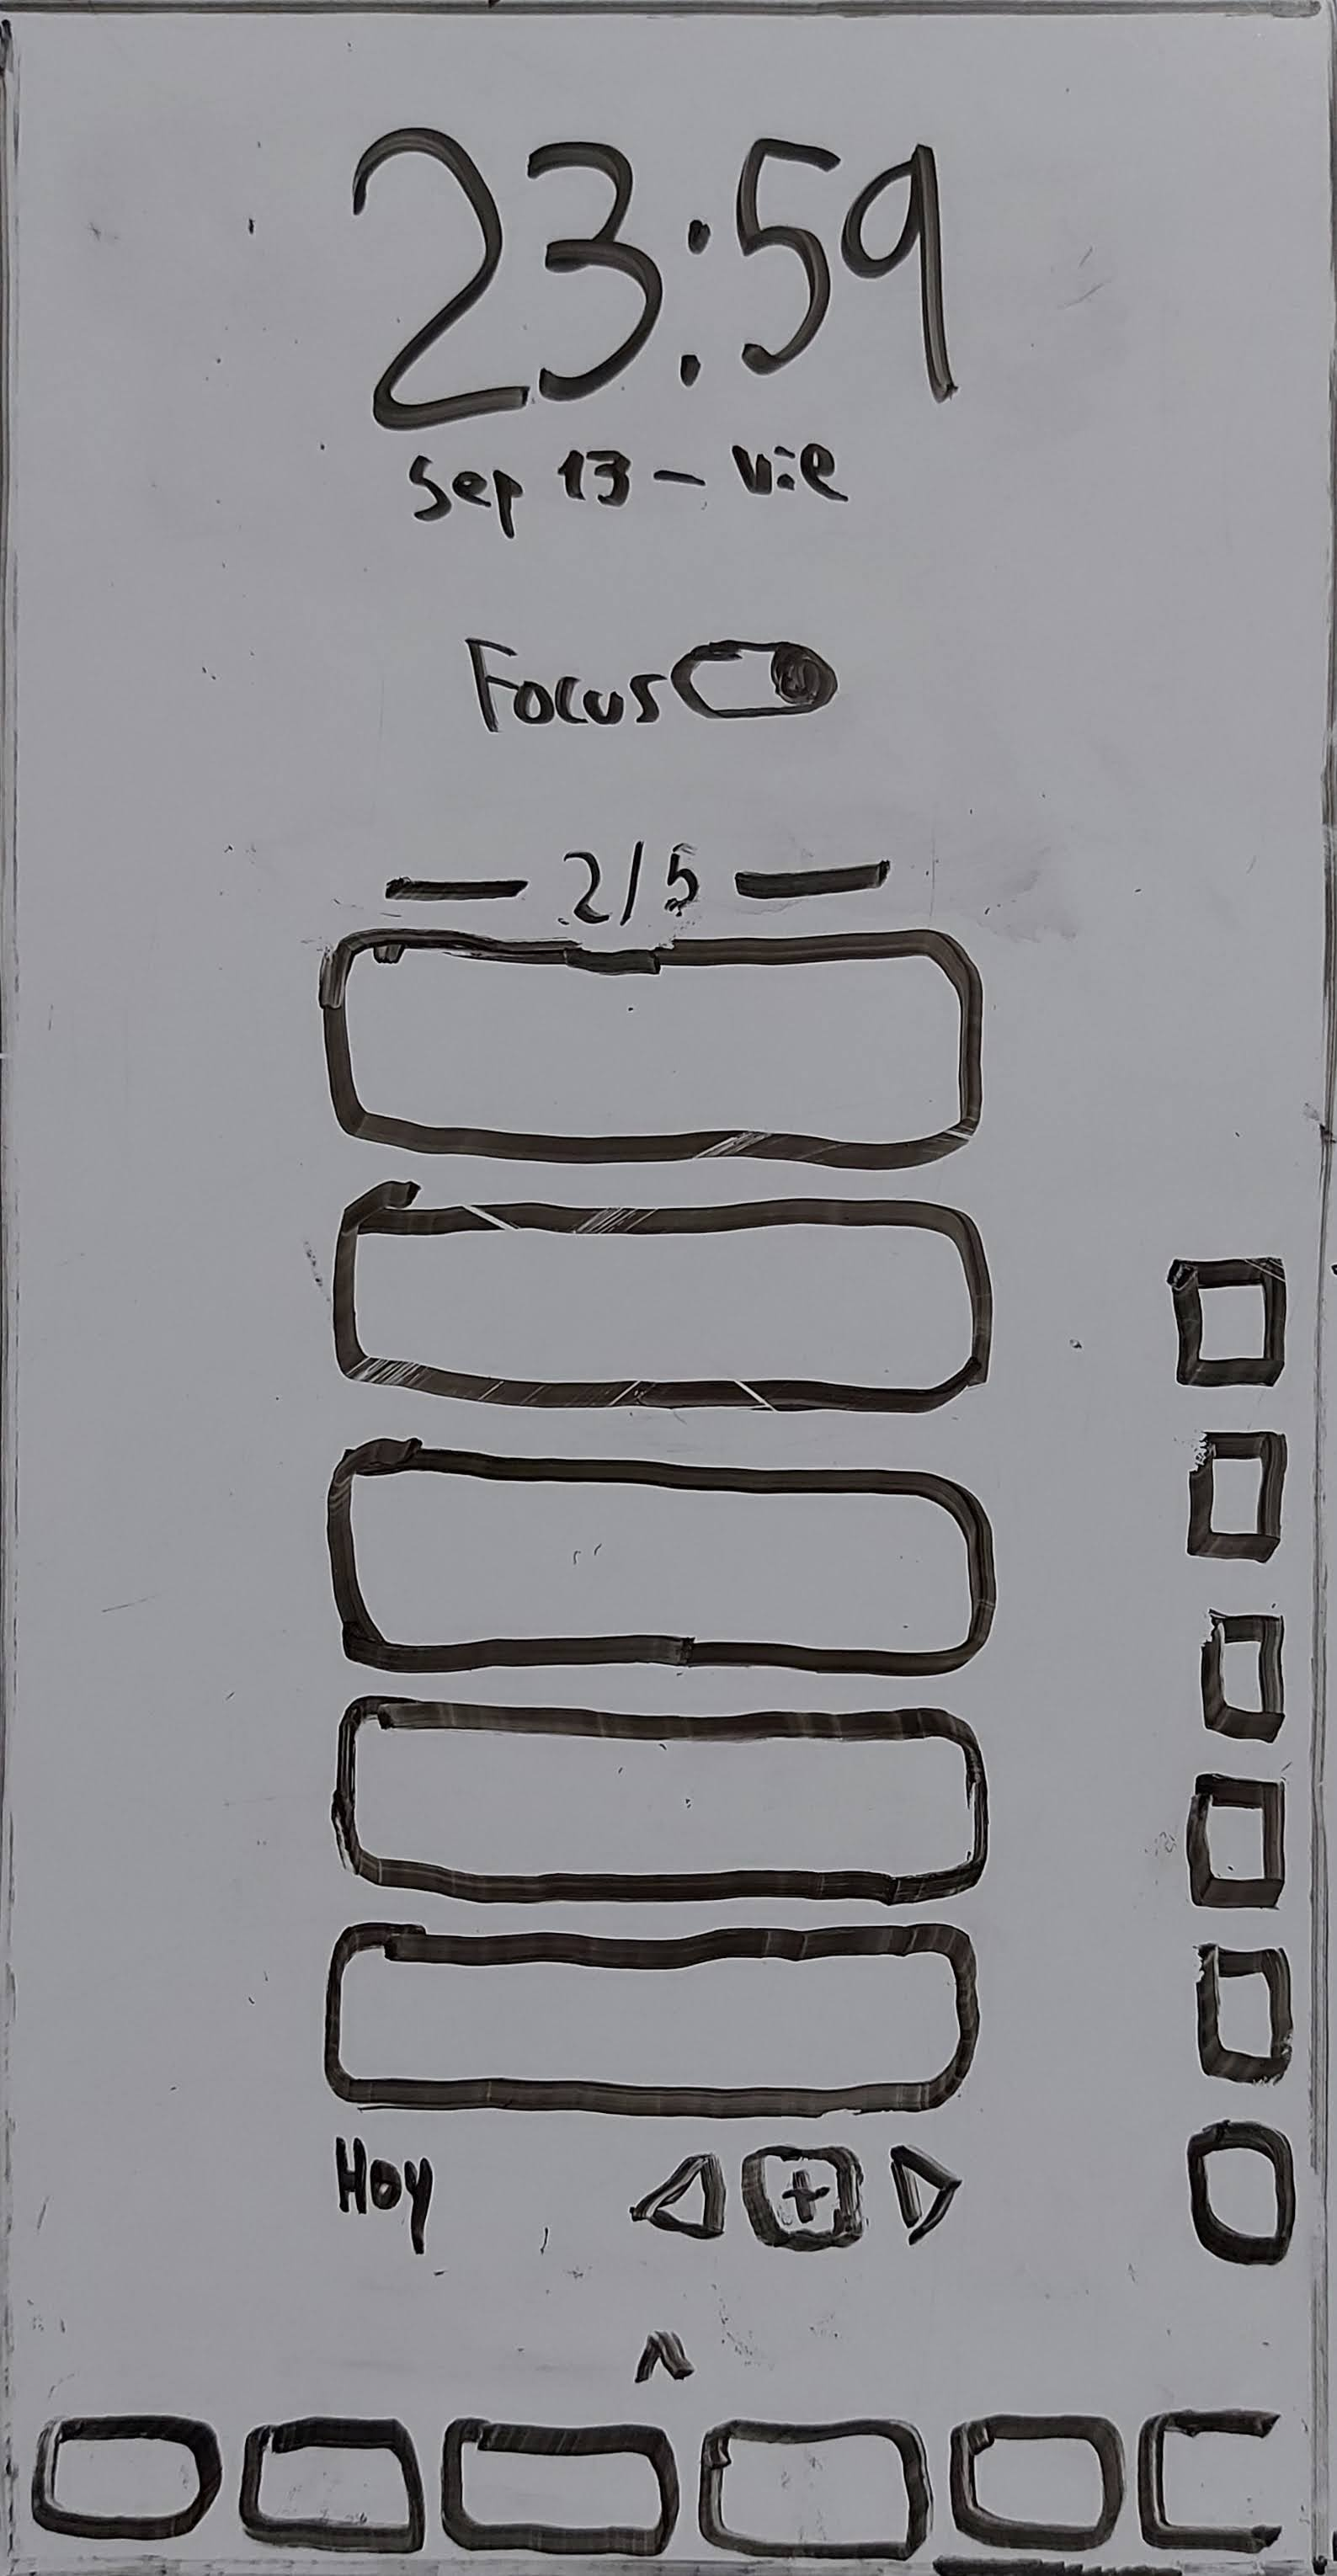
\includegraphics[width=0.5\textwidth]{Figuras/wireframe.jpg}
  \centering
\end{figure}


Una vez definidos los conceptos principales y validadas las ideas en el tablero físico, el proceso evolucionó hacia la creación de wireframes de alta fidelidad utilizando Figma. Esta transición permitió refinar los diseños con mayor precisión y establecer dimensiones específicas para los elementos de interfaz.

\begin{figure}[H]
  \caption{Wireframe de alta fidelidad.}
  \label{fig:wireframe_alta_fidelidad}
  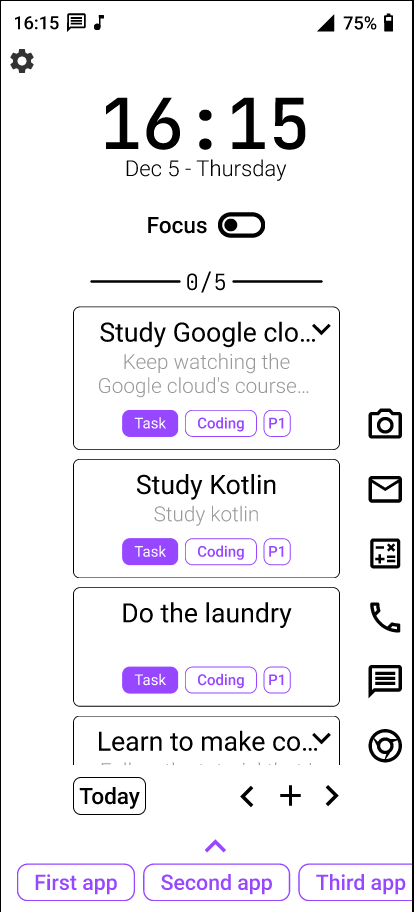
\includegraphics[width=0.5\textwidth]{Figuras/wireframe_alta_fidelidad.png}
  \centering
\end{figure}

La fase final del proceso de diseño consistió en la transformación de los wireframes de alta fidelidad en mockups prototipados que incorporaran todos los aspectos visuales del diseño final. Esta etapa incluyó la definición de la paleta de colores, tipografías, espaciados, proporciones, íconos, acciones y animaciones. Se buscó crear una interfaz que no solo fuera visualmente agradable, sino que también facilitara la interacción del usuario con las funcionalidades clave del launcher, como la gestión de tareas, hábitos y límites. Adicionalmente, se proyectó que la aplicación estuviera disponible en \textbf{español e inglés}, implementación realizada durante el desarrollo del proyecto. Los mockups y su prototipo se encuentran en \url{https://www.figma.com/design/EbtSyFZ1OGdiSgzbMcXiMW/Mockups?node-id=214-3438&t=4SbJQopzfLf274FE-1}.

\begin{figure}[H]
  \centering
  \begin{minipage}{0.48\textwidth}
    \caption{Mockup: Pantalla principal.}
    \label{fig:mockup_pantalla_principal}
    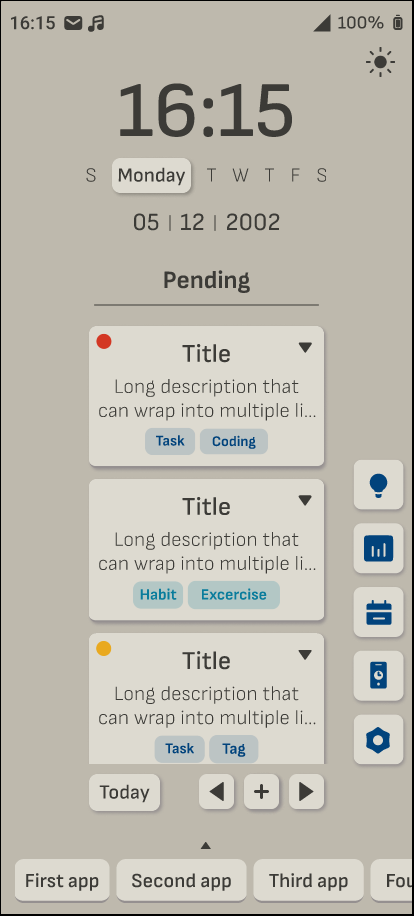
\includegraphics[width=\textwidth]{Figuras/mockup_1.png}
    \centering
  \end{minipage}\hfill
  \begin{minipage}{0.48\textwidth}
    \caption{Mockup: Pomodoro.}
    \label{fig:mockup_pomodoro}
    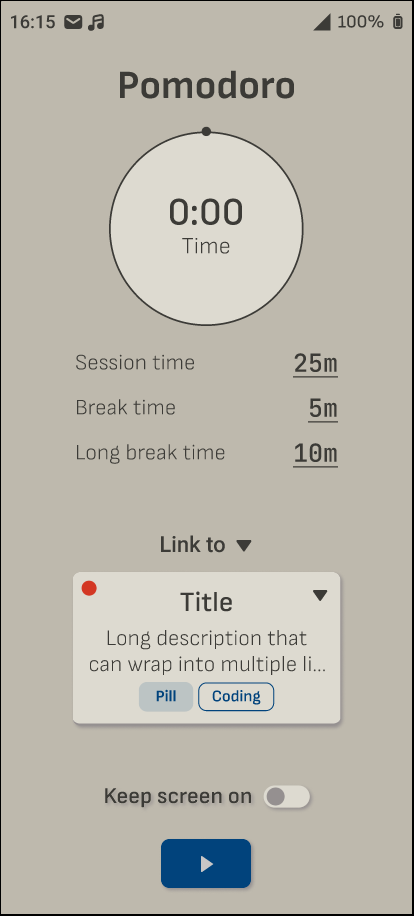
\includegraphics[width=\textwidth]{Figuras/mockup_2.png}
    \centering
  \end{minipage}
\end{figure}

\begin{figure}[H]
  \centering
  \begin{minipage}{0.48\textwidth}
    \caption{Mockup: Menú de aplicaciones.}
    \label{fig:mockup_menu_aplicaciones}
    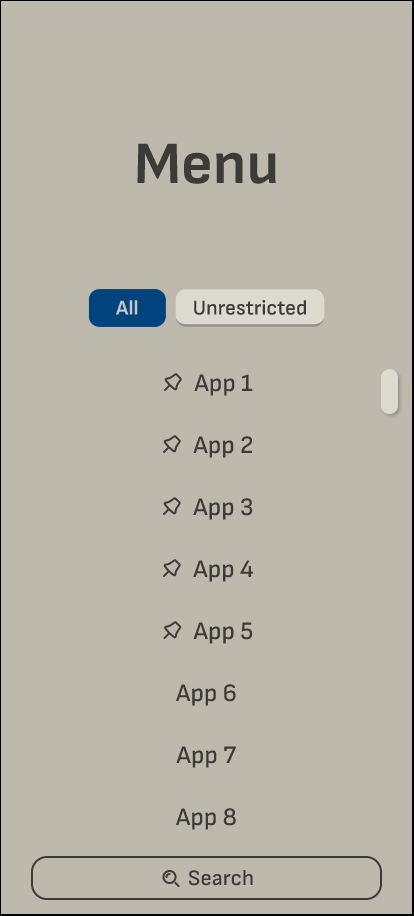
\includegraphics[width=\textwidth]{Figuras/mockup_3.png}
    \centering
  \end{minipage}\hfill
  \begin{minipage}{0.48\textwidth}
    \caption{Mockup: Configuraciones.}
    \label{fig:mockup_configuraciones}
    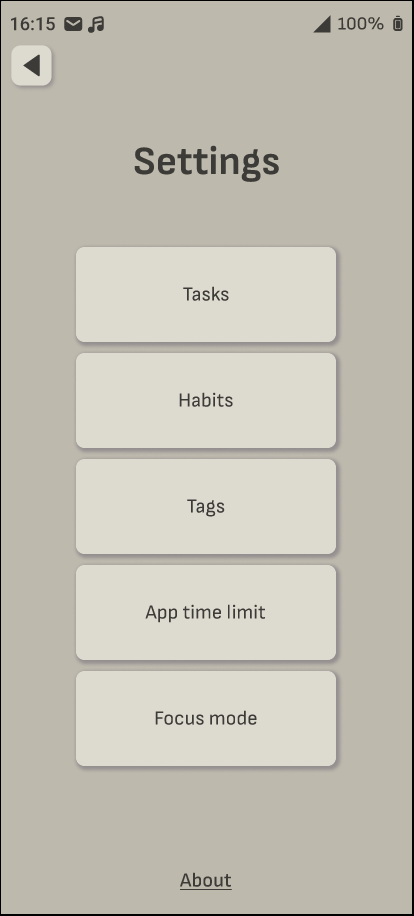
\includegraphics[width=\textwidth]{Figuras/mockup_4.png}
    \centering
  \end{minipage}
\end{figure}